\section{Implementation}\label{sec:imp}

For purposes of presentation, we have described an idealized and
unoptimized algorithm.  Our actual implementation includes a number of
refinements to improve the quality of the description and/or reduce the
inference time.  In this section, we discuss some of these refinements.

\subsection{Token families}
So far, parsing a \cd{Sync} token yields
one of three results: \cd{Good}, \cd{Fail} or \cd{Recovered}. 
In the actual implementation, a \cd{Sync} token can be not only a constant string, but also
a constant integer, an integer range or a combination thereof.
Consider parsing the token \cd{Sync (Str "GET")} when
the current input starts with ``POST.'' The
\cd{parse\_base} function indicates the result should be \cd{Fail}.
In reality, the input ``POST'' is in the same {\em family} as ``GET,'' 
\ie{}, a word,
and it may very well be that this \cd{Sync} token should have been 
an enumeration of words rather than a single word.
To handle such cases, we created a fourth type of parse node, \cd{Partial}, 
to indicate that the input belongs to the same family as the expected
token but does not match exactly, \ie, it is {\em partially} correct.
During aggregation, partial nodes cause the description 
to be specialized to include the additional values.  In the above example, the aggregate 
function will change the description to \cd{Sync (Enum [Word "GET", Word "POST"])}.
Such partial nodes reduce the number of parsing errors
and produce more compact and meaningful descriptions.

%% \subsection{Deterministic parsing}
%% In section \ref{sec:parse}, we presented a non-deterministic parsing semantics
%% for unions and arrays. While this is a correct semantics, it is expensive
%% to implement and is different from the \pads{} semantics of these two 
%% types.
%% Therefore in the prototype system, parsing a union involves 
%% attempting to parse the first branch and,
%% if it has error, attempting the second branch. This type of union semantics
%% is known as {\em deterministic choice}, as opposed to a non-deterministic
%% choice where both branches are always attempted.
%% When parsing an array, we use {\em longest match} semantics,
%% which means the parsing of the array elements and separators
%% continues until no more progress can be made in
%% the input. We will not elaborate these semantics because of lack of space.

\subsection{MDL score and description rewriting}
In the prototype system, we define the MDL score for a particular
\pads{} description \cd{D} as:
\[mdl\_score(D) = \costdescription{D} + w \times \acostdata{D}{x_1, \ldots, x_k},\]
where $\costdescription{D}$ is the type complexity of \cd{D}, defined in
\cite{Fisher+:dirttoshovels}, and
$\acostdata{D}{x_1, \ldots, x_k}$ is the atomic data complexity of 
data records $x_1, \ldots, x_k$ \cd{D} given that they can be described by
\cd{D}. We can think of the atomic data complexity as the number of bits 
to transmit an {\em average} data record given that 
we already have a description \cd{D}.
The MDL score of \cd{D} is basically the weighted sum of the two components,
and the weight is empiracally determined to be 10.

\begin{figure}[t]
\begin{center}
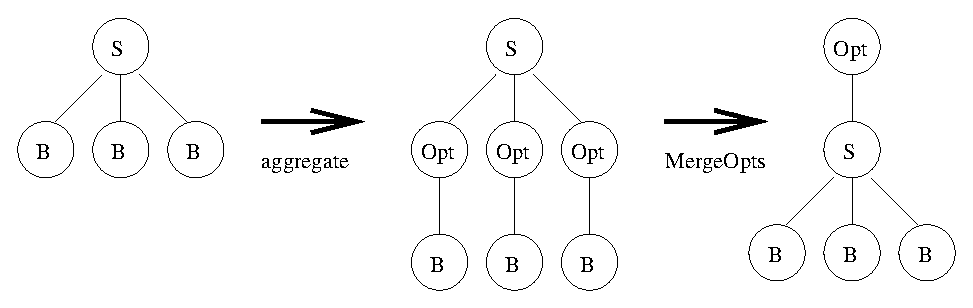
\includegraphics[width=\columnwidth]{opts}
%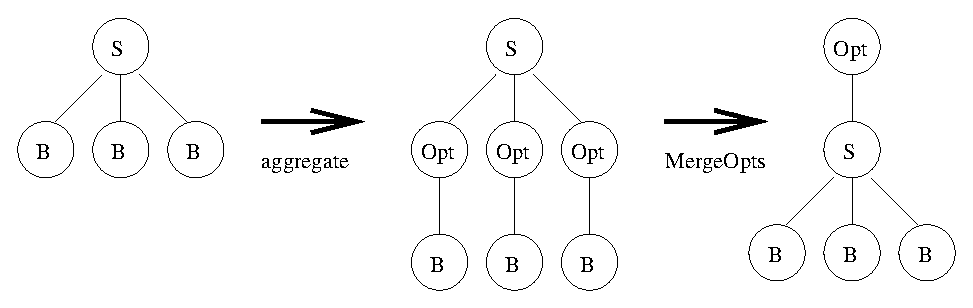
\epsfig{file=opts.eps,width=\columnwidth}
\caption{MergeOpts rewriting rule}\label{fig:opts}
\end{center}
\vskip -2ex
\end{figure}

When the incremental learning algorithm produces a refined description
from an aggregate, the algorithm applies rewriting rules
to the new description to improve its quality and readability.
Most of the rules are data-independent and inherited from \learnpads{}, such as 
removing degenerate lists and flattening nested structs and unions.

One data-independent rule that we added was {\em BlobFinding}. 
This rule takes a given sub-description \cd{D} and uses a heuristic to 
determine if it is over-verbose and needs to be simplified. 
The heuristic is that if the height of \cd{D} is larger than \cd{minBlobHeight}
(which is empiracally determined), and there is a special constant string 
or pattern \cd{re} immediately following
\cd{D} in the whole description, then we rewrite \cd{D} to 
\cd{Pstring\_SE(:re:)}.
\cd{Pstring\_SE} is a \pads{} base type that is similar to \cd{Pstring},
except it uses a stopping regular pattern as opposed to a stopping character
to mark the termination of a string. One thing to note is that a rewriting
rule is only effective if its resulting new description has a better MDL
score. That condition is implicit in the case of \cd{BlobFinding} rule, too.

We also introduce a new {\em data dependent} rule called {\em MergeOpts}
to optimize a type pattern that occurs frequently during incremental
learning.  Recall that the aggregate function
introduces \cd{Opt} nodes above a \cd{BaseA} or \cd{SyncA} node 
whenever the corresponding \cd{Base} or \cd{Sync} token in 
the description failed to 
parse. When faced with an entirely new form of data, 
the algorithm is likely to introduce a series of \cd{Opt} nodes as
each type in the original description fails in succession. 
The {\em MergeOpts} rule collapses these consecutive \cd{Opt} nodes if they
are correlated, \ie{}, either they are all always present or all always
absent.  To verify this correlation, the algorithm maintains a
table that records the branching decisions when parsing each
data line. It uses this table to determine whether to merge
adjacent \cd{Opt} nodes during rewriting. 
\figref{fig:opts} illustrates the effect of this rule.  In the figure,
$S$ denotes a struct and $B$ a base token.

\subsection{Initial batch and incremental batches}
We mentioned in Section \ref{sec:algo}, that we can learn an initial
description from any $N$ records from the source. In the implementation,
we simply take the {\em first} $N$ records from the source. The potential
problem with this
is that the final description could be skewed toward the first part of the
data. We choose to do this nonetheless because we do not want to make 
the assumption that we have the whole data file before we start learning
the description.  Furthermore, instead of learning the error data and 
updating the description every $M$ records which is indicated in 
\figref{fig:inc-learning}, we defer this till we have seen $M$ bad records.
 This avoids invoking the \cd{update\_desc} function unnecessarily when
there is no error data.

\subsection{Performance}
The pseudo-code in \figref{fig:inc-learning} suggests the number of
aggregates is of the order $O(m ^ n)$, where $m$ is the maximum number of
parses for a line of input  and $n$ is the number of lines to
aggregate.  Clearly, this algorithm will not scale 
unless $m$ and $n$ are bounded.

We have implemented several optimizations to limit the number of 
parses and aggregates. First, we do not return all possible
parses when parsing a description component \cd{D}. 
Instead, we rank the parses by the parse metric $m$ that
measures their quality and return only the top $k$. 
Metric $m_1$ is better than $m_2$ if $m_1$ is perfect and $m_2$ is not, 
or if $m_1 > m_2$.

In practice, \cd{parse} returns a list of
{\em parse triples} $(r,~m,~j)$, where $r$ is the data representation of
the parse, $m$ is the metric associated with $r$, and
$j$ is the position in the input after the parse.
We define a \cd{clean} function that first partitions the
triples into groups that share the same 
{\em span}, \ie{}, the substring of the input consumed by the parse.
For each group, \cd{clean} retains all perfect parses. If 
none exists, it retains the best $k$ non-perfect parses in the group. 
We justify discarding the other triples because
given a description $d$ and a fixed span, we always
prefer the parse with the best metric. This idea is
similar to the dynamic programming techniques used in 
Earley Parsers \cite{earley-parser}. 

An interesting thought is what if
we set $k=1$, that is, allow only the best error parse if there is
no perfect parses. While this strategy significant reduces the
state space of the parsing and hence the aggregation operations,
it usually results in sub-optimal overall parse structure. Here is an
example. Suppose the current top level description \cd{D} when learning 
the \ai{} format is:
\begin{code}
\kw{Precord} \kw{Pstruct} entry_t \{
         Phostname      host;
   ' ';  
   '-';  /* the first dash */
   ' ';  
   '-';	 /* the second dash */   
   " ["; Pdate          date;
   ':';  Ptime          time;
   "] "; request_t      request;
   ' ';  Pint           response;
   ' ';  Pint           length;
\};
\end{code}
Note all constant strings or characters are used as sync tokens during
parsing. Now \cd{D} is used to parse the second record in \figref{fig:ai}.
\cd{D} parses the above data without error until it
reaches the second dash in \cd{D}. It expects a sync token
'-', but instead sees a string \cd{amnesty} in the input.
According to the semantics of sync token in \figref{fig:parse-sem},
there can be two possible parses:\\
{\footnotesize
\verb#(Recovered "kim [10/May/2009:18:38:35 ", (1, 26, 1))#\\
\verb#(Fail, (1, 0, 0))#
}

In the first parse, 26 characters are skipped before a \cd{-} is found.
In the second parse, a failure is returned and no characters are consumed
from the input.
By (\ref{eqn:metric-eqn}), the first parse is better and therefore the
second one is disgarded. Unfortunately, this strategy causes the parsing of the
remaining types up to \verb#"] "# to fail, thereby giving a bad overall parse.
If we keep the second parse and continue with it, the next sync token 
\verb#" ["# will be able to recover after skipping \cd{kim} and succeed
in parsing the rest of the types hence giving a better overall parse.
Therefore in the implementation, we set $k$ to be a small number but larger
than 1.

A second optimization, which we call {\em parse cut-off}, terminates a
candidate parse when parsing a struct with multiple
fields $f_1$, $f_2$, ..., $f_n$ if the algorithm encounters 
a threshold number of errors in succession. 
This technique may result in no possible parses for the
top-level description.  In this case, we restart the process
with the parse cut-off optimization turned off. 
A third optimization is memoization.
The program keeps a global memo table indexed by the pair of a
description \cd{D} and the beginning position for parsing \cd{D} which
stores the result for parsing \cd{D} at the specific position.
Finally, we bound the total number of aggregates the
algorithm can produce by selecting the top
$k$ aggregates with the fewest number of \cd{Opt} and \cd{Learn}
nodes. 


